%!TEX root = /Users/Nikolaj/Developer/GPU-Project/Report/Report.tex
The following two sections describe the two CUDA implementations made during this project. The first attempt, MiddlePar, was the first iteration on how we could parallelize the mathematical model described in Section \ref{themath}. The second and final attempt, OuterPar, is an improved version of the first attempt that address the issues discovered in MiddlePar. Both CUDA implementations are derived directly from the C implementation described in Section \ref{implementation}.

\subsection{First Attempt: MiddlePar}
\label{sec:firstattempt}
In order to parallelize the C implementation and utilize the GPU, we had to analyze each model. Our approach was to locate the most obvious part that could be parallelized, and develop a CUDA version. Since not all computations could be parallelized, we acknowledged that some computation would be run on the CPU, and the rest would be run on the GPU. The most obvious possibility for a CUDA solution was found within the middle model. Contrary to both the outer and the inner model, each step within the middle model was not dependent on the previous step in the same model. A step in \texttt{Middle} is calculated by adding the weighted average of $k1$, $k2$, $k3$, $k4$ to the $y$-value of the previous step. This means that for each step we can calculate the weighted average of all the $k$ values before we add the corresponding y value. This is a good start since the calculation of each $k$, is essentially a call to the inner model. The MiddlePar implementation is explained in the following section.

\subsubsection{MiddlePar Implementation}
The implementation of the kernel is invoked in the method \texttt{OuterDiff}, which is the method that needs a result from the middle model. \texttt{OuterDiff} prepares two variables that is copied to the GPU. The first is the current $x$-value from the outer model, that is needed to calculate \texttt{Middle}, and an array called \texttt{kSum}. \texttt{kSum} is used to store the weighted averages of $k1$, $k2$, $k3$ and $k4$, calculated by each thread. With these weighted averages, calculating each step in \texttt{Middle} can be done much faster, since it is only a matter of adding two double values together for each step. \\

Based on the stepsize it is possible to calculate exactly how many steps \texttt{Middle} needs to take. Prior to starting the kernel, we need to make sure that there are enough threads available, such that there are at least one thread for each step. The amount of threads per block is set prior to program execution, and before starting the kernel, the amount of blocks needed to ensure enough threads is automatically calculated.

\begin{figure}[ht!]
\begin{lstlisting}[language=c]
__global__ void Middle(double *t, double *kSum){
	int tid = threadIdx.x + blockIdx.x*blockDim.x;
	//constData[4] refers to the h2 constant
	double stepsize = -1 / constData[4]; 
	//constData[6] refers to the level2fullsteps constant
	const int fullsteps = constData[6]; 
	if(tid<fullsteps){
		double gt = *t; //de-reference input
		//constData[0] refers to the x constant
		double tau = constData[0] + gt; 
		double kk = k(tau);
		double eta = (120+(tid*stepsize));
		double k1 = stepsize * MiddleDiff(tau, eta, Inner(eta, gt, kk).y);
		double k2 = stepsize * MiddleDiff(tau, eta + stepsize/2, Inner(eta + stepsize/2, gt, kk).y);		
		double k4 = stepsize * MiddleDiff(tau, eta + stepsize, Inner(eta + stepsize, gt, kk).y);
		kSum[tid] = k1/6+k2/3+k2/3+k4/6;
	}
}
\end{lstlisting}
\caption{The kernel code for \texttt{Middle} in MiddlePar}
\label{fig:middlepar}
\end{figure}

The implementation can be seen in Fig. \ref{fig:middlepar}. Once the kernel has been started, each thread calculates their global thread id as $threadIdx.x + blockIdx.x \times blockDim.x$. This ensures that each thread within the kernel has a unique id.\\

We then ensure that only threads, that have an id within the range of middle steps, continue on from line 7 in Fig. \ref{fig:middlepar}. We know that this might cause branch divergence in the last block if the total amount of threads is not equal to the amount of steps. However this is a necessary precaution as the size of \texttt{kSum} is exactly the total amount of steps, so if a thread id is larger than this, we risk writing data to unallocated memory. A solution could be to always make sure that the number of threads you have is equal to the amount of steps to be taken, however since both threads per block, as well as middle steps, varies it is not feasible, and cannot always be ensured.\\

The next couple of lines is used to calculate local variables, that is used to call both \texttt{Inner} and \texttt{MiddleDiff}. $k1$, $k2$ and $k4$ is then calculated by calling \texttt{MiddleDiff} and \texttt{Inner}. In line 16 in Fig. \ref{fig:middlepar} the weighted average of each $k$ is calculated and stored in the \texttt{kSum} array. This is where it is important that the thread id does not exceed the amount of steps. Once the sum of the $k$ values have been stored in \texttt{kSum} for all threads, the kernel terminates. The result is copied back to the CPU, where the sum of the array is computed as shown in Fig. \ref{fig:middleparcpu}. The program then continues as normal.

\begin{figure}[ht!]
\begin{lstlisting}[language=c]
//Copy the result of running the kernel back to the CPU
cudaMemcpy(kSum, d_kSum, level2fullsteps*sizeof(double), cudaMemcpyDeviceToHost);

point nextPoint = {120.0,0.0};
double y = nextPoint.y;
int i;
for(i = level2fullsteps-1; i>=0; i--){
	y = y+kSum[i];
}
\end{lstlisting}
\caption{The CPU code in \texttt{OuterDiff} that sums the values of \texttt{kSum}}
\label{fig:middleparcpu}
\end{figure}

The execution flow of the MiddlePar implementation is shown in Fig. \ref{fig:middleparexec}.

\begin{figure}[ht!]
  \centering
    \includegraphics[scale=0.5]{ProgramexecutionMiddlePar}
  \caption{Execution flow: MiddlePar implementation}
  \label{fig:middleparexec}
\end{figure}

\subsubsection{MiddlePar Memory Considerations} \hfill \\
This implementation frequently accesses the number of steps per year when calculating \texttt{Inner}. Since we only read this constant, it makes sense to place this variable in constant memory. Constant memory is considerably faster than global memory\cite{bpg} because it has it's own cache, with the limitation that you cannot alter the data.\\

It was also considered to keep \texttt{kSum} in shared memory. Shared memory allows threads within the same block to share data, but not between blocks. Shared memory, like constant memory, is considerably faster than global memory, however it is possible to use in this implementation as any thread from any block needs to access the array.

\subsubsection{MiddlePar Shortcomings} \hfill \\
\label{label:shortages}
The implementation described in Section \ref{sec:firstattempt} has a few shortcomings:
\begin{enumerate}
	\item Each time a call to \texttt{Middle} is made, variables is copied to the GPU and a new kernel would be started. Creating a large number of kernels that terminates quickly introduces a lot of overhead. In MiddlePar this is the case when the values for $x$ and $h$ are high.
	\item The implementation potentially needs more than one block to parallelize the steps \texttt{Middle} if the amount of threads per block are low. Even though it does parallelize each step in \texttt{Middle}, the calls to \texttt{Middle} are still sequential.
	\item We are not exploiting all available SMP's as shown by the profiler and described in Section \ref{sec:profiler}.
	\item It would be much more efficient to use shared memory for storing the \texttt{kSum} array, instead of keeping it in global memory.
\end{enumerate}

\subsection{Second Attempt: OuterPar}
To address the shortcomings of the MiddlePar implementation, we made some major changes to the existing GPU and CPU code. First we made sure that \texttt{Middle} was only being calculated using the threads within a single block. We also changed \texttt{kSum} to be a shared variable array instead of a kernel parameter. \\

Furthermore we parallelized the calls to \texttt{Middle}. A closer look at the outer model showed that the different calculations of \texttt{Middle} in every outer step depended only on one variable; the current $x$-value. This effectively meant that we could calculate all $x$-values used by \texttt{Middle} before the kernel was invoked since the stepsize $h$ and the initial and final $x$-value was known. Using these $x$-values we could calculate all calls to Middle in parallel. Together with the changes to \texttt{Middle} this allowed us to use different blocks to calculate different calls to \texttt{Middle} at the same time and better utilize the GPU resources. The OuterPar implementation is described in the following section.

\subsubsection{OuterPar Implementation} \hfill \\
The first changes to \texttt{Middle} were to modify the calculation of the thread id as shown in line 3 and change kSum to a shared variable as shown in line 2 in Fig. \ref{fig:outerpar}. The changes were made to address two of the issues described in \ref{label:shortages}, regarding the use of multiple blocks within a single call \texttt{Middle(…)}, as well as the lack of a shared variable to store \texttt{kSum}. Fig. \ref{fig:outerpar} shows the updated code.

\begin{figure}[ht]
\begin{lstlisting}[language=c]
__global__ void Middle(double *outerx, double *temp){
	extern __shared__ double kSum[];
	int tid = threadIdx.x;
	double stepsize = -1 / constData[4];
	const int fullsteps = constData[6];
	double gt = outerx[blockIdx.x];
	while(tid<fullsteps){
		double tau = constData[0] + gt;
		double kk = k(tau);
		double eta = (120+(tid*stepsize));
		double k1 = stepsize * MiddleDiff(tau, eta, Inner(eta, gt, kk).y);
		double k2 = stepsize * MiddleDiff(tau, eta + stepsize/2, Inner(eta + stepsize/2, gt, kk).y);		
		double k4 = stepsize * MiddleDiff(tau, eta + stepsize, Inner(eta + stepsize, gt, kk).y);
		kSum[tid] = k1/6+k2/3+k2/3+k4/6;
		tid = tid + blockDim.x;
	}
	tid = threadIdx.x;
	__syncthreads();
	if(tid == 0){
		double y = 0.0;
		int i;
		for(i = fullsteps-1; i>=0; i--){
			y = y+kSum[i];
		}
		temp[blockIdx.x] = y;
	}
}
\end{lstlisting}
\caption{The kernel code for \texttt{Middle} in the OuterPar implementation}
\label{fig:outerpar}
\end{figure}

The next change is that we get the $x$-value from the outer model, from a pre-calculated array, \texttt{outerx} holding all the $x$-values used in \texttt{OuterRK}. This array is passed to the kernel at execution time. The $x$-value needed for a specific block can then be accessed using the unique block id as an index the the array shown in line 8 in Fig. \ref{fig:outerpar}).\\

We further changed the if-statement in line 7 in Fig. \ref{fig:middlepar} to a while-loop in line 7 in Fig. \ref{fig:outerpar} and added a counter in line 15. Since the number of threads per block could be less than the number of steps to be taken, we wanted to ensure that threads iterated over multiple steps instead of just one, such that \texttt{kSum} would be correctly filled. It also ensured that if a block contained more threads than there were steps to be taken, they would not enter the while loop. Apart from the counter, everything within the while loop is the same as in Fig. \ref{fig:middlepar}.\\ \\

The code found in line 17-26 in Fig. \ref{fig:outerpar} was originally placed in \texttt{OuterDiff} in the MiddlePar solution. The reason for this, was that we used multiple blocks for the same \texttt{Middle} call, one could never guarantee that all blocks had reached the same part of the code before moving on. The only situation where it was certain that all blocks have finished execution was when the kernel terminated. In the MiddlePar solution we therefore copied \texttt{kSum} back to the CPU and made it compute the sum there. However, now that we are only working within a single block we can make use of the \texttt{\_\_syncthreads()} statement (line 18 in Fig. \ref{fig:outerpar}) and compute the sum on the GPU. The \texttt{\_\_syncthreads()} statement ensures that all threads (within the same block) have reached this line of code before computing the sum. We also reset the thread id in line 17 in Fig. \ref{fig:outerpar}.\\

Once the weighted average of $k1$, $k2$, $k3$ and $k4$ has been calculated for each thread we need to sum them. There are basically two ways to do this; use a single thread to iterate over all the values in \texttt{kSum} and sum them, or use reduction \cite{byexample}. Reduction is a method that makes use of the threads already available, and have them add two values until you only have one value is left. See Fig. \ref{fig:reduction} for a visualization of this concept. This allows the sum of \texttt{kSum} to be computed in $log_2 (threadsperblock)$ iterations.\\

\begin{figure}[ht!]
  \centering
    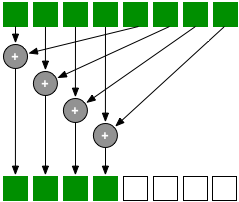
\includegraphics[scale=0.5]{Reduction}
  \caption{The principle of reduction \cite{byexample}}
  \label{fig:reduction}
\end{figure}

Reduction seems like the most obvious choice, however, the size of the array and the number of threads is the power of two, \cite{byexample}. We can make sure that the number of threads per block is always a power of 2, however we can never guarantee that the same holds for the size of \texttt{kSum}. The size of \texttt{kSum} is $\frac{119}{h}$, and this cannot be guaranteed to be the power of 2. A solution to this would be to always make sure that the size of \texttt{kSum} is the power of 2, and fill the unused indexes with zeros. However, the increase i performance were neglectable compared to the total calculation of a \texttt{Middle} call. We therefore decided not to use reduction in this case.\\

Once the sum has been calculated it is stored in a temporary array holding the sum from each block. Once all blocks have computed their sum, the kernel terminates and the temporary array is copied back to the CPU. When \texttt{OuterRK} is called, instead of calling \texttt{Middle} it indexes into temporary array. The code for calculating the initial \texttt{outerx} array for the kernel is shown in Fig. \ref{fig:outerparcpu}.

\begin{figure}[ht!]
\begin{lstlisting}[language=c]
//Prepare an array of all possible x values
int stp = 0;
int b; //fullstep counter
for(b = 0; b <= size; b++)
{
	//Take full step
	if(b%2 == 0){
		steps[b] = (120-x) + stp*(-1.0/h1);
	}
	//Take half step (value needed in OuterRK)
	else{
		steps[b] = ((120-x) + stp*(-1.0/h1))+((-1.0/h1)/2);
		stp += 1;
	}
}
\end{lstlisting}
\caption{The CPU code in \texttt{Outer} for calculating all needed $x$-values in advance.}
\label{fig:outerparcpu}
\end{figure}

The execution flow of the MiddlePar implementation is shown in Fig. \ref{fig:outerparexec}.

\begin{figure}[ht!]
  \centering
    \includegraphics[scale=0.5]{ProgramexecutionOuterPar}
  \caption{Execution flow: OuterPar implementation}
  \label{fig:outerparexec}
\end{figure}

\subsubsection{OuterPar Memory Considerations} \hfill \\
Just like the MiddlePar implementation, this implementation frequently accesses a constant variables when calculating \texttt{Inner}, but for this implementation it also accesses the constants $x$, $h$ and $level2fullsteps$, holding the number of fullsteps in \texttt{Middle}. Since we only read these constants we kept them in constant memory.\\

However compared to the MiddlePar solution \texttt{kSum} was now kept in shared memory instead of global memory. Writing to this array should now be faster than the previous solution.

\subsection{Profiling and Comparison}
\subsubsection{Nvidia Visual Profiler Results} \hfill \\
\label{sec:profiler}

We used Nvidias Visual Profiler to analyse the MiddlePar and OuterPar implementation. We present the results in Table \ref{table:profiler} and discuss them in the next section.

\begin{savenotes}
\begin{table}  
\begin{center}
\begin{tabular}[t]{|c|c|c|}
	\hline
\textbf{Attributes} & \textbf{MiddlePar} & \textbf{OuterPar} \\\hline
Grid size  & 2,1,1 & 1700,1,1\\\hline
Block size & 128,1,1&128,1,1\\\hline
Registers/thread & 62&63\\\hline
Shared Memory/Block &0 bytes& 1904 bytes\footnote{The visual profiler wrote that OuterPar used 1859 bytes of shared memory. This is however wrong. The command line profiler showed the correct result. The result can be calculated as $119 \times h2 \times 8$, which in this case is $119 \times 2 \times8$ = 1904 bytes.}\\\hline
Global Load Efficiency\footnote{We assume that we can achieve max 100\% efficiency.}&86,2\%&764.5\%\\\hline
Global Store Efficiency&99,2\%&25\%\\\hline
Branch Divergence Overhead&21.9\%& 21.8\%\\\hline
Occupancy\footnote{According to the profiler the theoretical occupancy is 33.3\%.}&6.5\%&33.1\%\\\hline
\end{tabular}
\end{center}
\caption{Nvidia Profiler Results. Input: $g=10$, $r=65$, $x=35$, $h1=10$, $h2=2$, $h3=10$, $threadsPerBlock=128$.}
\label{table:profiler}
\end{table}
\end{savenotes}

Apart from these attribute values the following warnings were issued by the profiler:
\begin{itemize}
	\item MiddlePar
	\begin{enumerate}
		\item \textbf{Low Multiprocessor Occupancy}. Limited grid size prevents the GPU from using all available SMP's.
		\item \textbf{High Branch Divergence Overhead}. Divergent branches can cause significant instruction issue overhead.
		\item \textbf{Inefficient Memcpy size}. Small memory copies do not enable the GPU to fully utilize the host to device bandwidth.
		\item \textbf{Low Memcpy Throughput}. The memory copies are not fully using the available host to device bandwidth.
	\end{enumerate}
	\item OuterPar
	\begin{enumerate}
		\item \textbf{High Branch Divergence Overhead}. Divergent branches can cause significant instruction issue overhead.
		\item \textbf{Low Memcpy Throughput}. The memory copies are not fully using the available host to device bandwidth.
	\end{enumerate}
\end{itemize}

\subsubsection{Comparison and Discussion} \hfill \\
It is evident from the results in Table \ref{table:profiler} that there are major differences between the two implementations, namely grid size, occupancy and global store effiency.
\\ \\
The difference in grid size makes sense, when considering the implementation differences. MiddlePar parallelizes a single call to \texttt{Middle}, whereas \texttt{OuterPar} computes all middle calls in parallel. 
%The number of blocks in MiddlePar depends on the number of threads per block, and the number of steps to be taken in middle model. In the worst case, this would require 38 blocks to cover a middle stepsize of 10 and 32 threads per block\footnote{If the steps per year is 10 we need to take $119 \times 10$ steps, and with 32 threads per block we would need ceil($frac{119 \times 10}{32}$) blocks to cover all steps.}. This stands in large contrast to the amount of blocks used by OuterPar. 
The difference is that MiddlePar creates a large number of kernels when executing the program, whereas OuterPar creates a single kernel.\\

From this, the difference in occupancy is also evident. While MiddlePar runs a large number of kernels in sequence with a small number of blocks, OuterPar runs a single kernel with a large number of blocks. This means that the total number of threads running at any time is larger in the OuterPar implementation than in the MiddlePar implementation. If the number of blocks that are running simultaneously is not enough to occupy all the SMPs available, the occupancy will fall. Therefor is it natural that the OuterPar implementation has a higher occupancy than the MiddlePar implementation. \\

%Running a very small number of blocks with a small number of threads is only going to use a small part of the GPU. Furthermore whenever warps fetch data from global memory during the MiddlePar execution, storing to global memory waiting for a flop to finish, there are almost no warps to take its place while it waits. This means that the SMP's that have blocks assigned will be idle (further lowering occupancy). During OuterPar execution there are enough blocks to assign the full number of blocks per SMP on the GPU. Furthermore whenever a block finishes execution, there are several blocks waiting to be assigned to a SMP leaving very little time to stand idle. The time the SMP's will start to idle will begin towards the end when there are no more blocks waiting in the pipeline. All together this means that the GPU will be fully occupied during most of the kernel execution.

Global store efficiency is different for the two programs for a simple reason. Where most of the threads in MiddlePar writes to global memory, only a single thread per block writes to global memory in OuterPar. Whenever a request to write to global memory is initiated the SMP tries to write the minimum amount of bytes possible which is 32 bytes. Since we are only storing a single double value (8 bytes), only 25\% of the store request is actually used. \\

The warnings issued by the profiler clearly indicates that the implementation not fully utilizing the bandwidth between the host and the device. For MiddlePar we only copy a small $kSum$ array back and forth between the host and device, which  includes $119(years) \times 10(steps per year) \times 8(size of double) = 9420$ bytes for a $h$ of 0.1. For OuterPar it contains at most $120(years) \times 10(steps per year) \times 2(half steps included) \times 8(size of double) = 19200$ bytes for the same $h$. Considering that the bandwidth between the host and device is 8 Gb/s we are not even close to the bound for either implementation, and therefore both implementations are compute bound, rather than memory bound.

\subsection{Possible Extension}
In the following we will describe an alternative extension on how to parallelize the C implementation. \\

The approach was to have the same setup as in OuterPar. The main difference would was the structure of \texttt{Middle(...)} on the GPU. Instead of having a single thread for each step in middle, there would be a thread for each $k$. This would mean that there would be three threads for each step in middle. With this approach only a single call to \texttt{Inner()} would be executed for each thread. The concept is illustrated in Fig. \ref{fig:alternative}.

\begin{figure}[ht!]
  \centering
    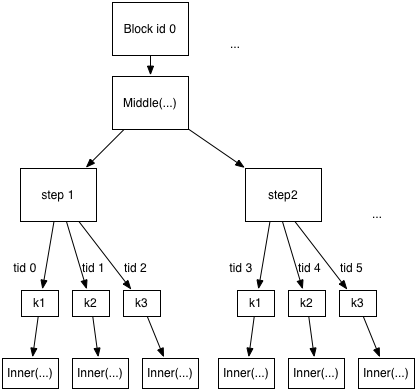
\includegraphics[scale=0.5]{alternative_solution}
  \caption{Alternative Solution}
  \label{fig:alternative}
\end{figure}

There is a limitation though. Even for a number of steps per year as small as 3, we would need $119(years) \times 3(steps per year) \times 3(ks) = 1071$ threads per block which is more than the hardware limit of 1024 threads per block. If we limit the number of threads per block to 1024 and keep a stepsize of 3, each thread would have to make more than one call to \texttt{Inner} which was what the OuterPar implementation was doing already. This means that as long as the number of threads per block needed to perform all the steps exceed the hardware limit of 1024, we do not gain any performance compared to the OuterPar implementation, in theory. \\

A second argument against the extension is that the size of the $kSum$ array would be three times larger than it is with the OuterPar implementation. The reason for this is that the array stored weighted averages in the OuterPar implementation, but with this extension the array would store a $k$ values. \\

%The last argument is that the $Middle$ method would have to calculate the weighted averages for each consecutive set of 4 k indices. Furthermore, the initial array containing the x values used to to calculate the different k vlaues would have to be constructed in such a way that each thread would use the right x value 

%There is a limitation though. Since we will be using 3 threads per step in middle, completing all the steps without looping, for even $stepsize = 2$ would require at least 714 threads, for $stepsize = 3$ 1071 threads, for $stepsize = 4$ 1428 threads and so on. We would then be forced to loop with each thread since we would very quickly reach the limit of 1024 threads per block. Given a large enough $stepsize$ each thread would have to do as many calls to \texttt{Inner()} anyway. Furthermore the shared $kSum$ variable would have to be three times larger since it would not be possible to calculate the weighted sum before all threads were done. The complexity of handling all these issues were deemed to be inferior to the much simpler approach in the current OuterPar solution. \\

The implementation was discarded already in the design phase because of the arguments stated above.
